%%%%%%%%%%%%%%% preamble %%%%%%%%%%%%%%%%%%%%%%%
\documentclass{article}
\usepackage{geometry}
\geometry{a4paper}
\usepackage{graphicx}
\usepackage{framed}
\usepackage{xcolor}
\usepackage{hyperref}
\usepackage{tikz}
\usetikzlibrary { decorations.pathmorphing, decorations.pathreplacing, decorations.shapes,
}
\usepackage{wela}
\usepackage[T1]{fontenc}
%%%%%%%%%%%%%%%%%% preamble %%%%%%%%%%%%%%%%%%%%%%
\begin{document}
\title{Writing About Charts, Diagrams, and Tables}
\date{}
\maketitle
\begin{center}
	\includegraphics[trim = 5cm 25cm 4cm 1cm, clip, width=0.8\textwidth]{diagrams.pdf}
\end{center}
As an engineer or scientist, you may be required to analyse a given graph or report your own numerical results. Altough you will probably be biased to the terminology in your field of expertise, practicing this skill, in advance, gives you the confidence to dive into expressing yourself and convincing your audience. Here we practice some useful language for that purpose. For now, the bar chart in figure~\ref{fig:social} is our reference for providing examples. (That's the default, unless otherwise specified.)

\begin{figure}
	\center
	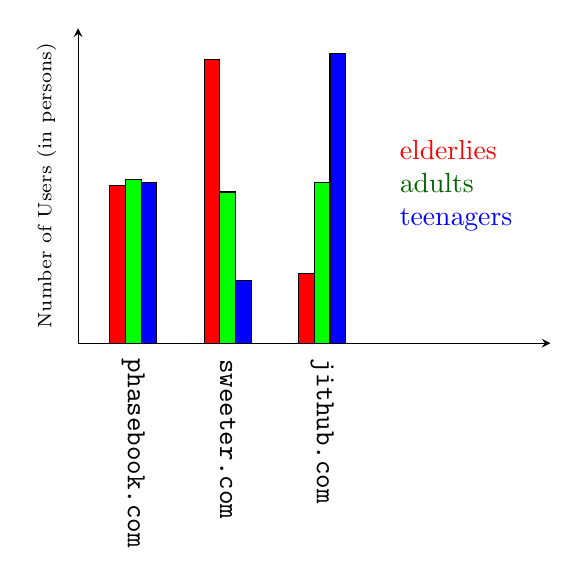
\begin{tikzpicture}[scale = 0.4]
		\draw[-stealth] (0,0) -- (0,10);
		\node[rotate=90] at (-1, 5) {{\scriptsize Number of Users (in persons)}};
		\draw[-stealth] (0,0)--(15,0);
		\node[align=left] at (12, 5) {\textcolor{red}{elderlies}\\\textcolor[rgb]{0,0.4,0}{adults}\\\textcolor{blue}{teenagers}};

		\draw[fill=red] (1,0) rectangle (1.5, 5);
		\node[rotate=-90] at (1.75,-3.5) {\texttt{phasebook.com}};
		\draw[fill=green] (1.5, 0) rectangle (2,5.2); 
		\draw[fill=blue] (2,0) rectangle (2.5, 5.1);


		\draw[fill=red] (4,0) rectangle (4.5,9);
		\draw[fill=green] (4.5,0) rectangle (5,4.8);
		\draw[fill=blue] (5,0) rectangle (5.5, 2);
		\node[rotate=-90] at (4.75, -3.05) {\texttt{sweeter.com}};

		\draw[fill=red] (7,0) rectangle (7.5, 2.2);
		\draw[fill=green] (7.5,0) rectangle (8,5.1);
		\draw[fill=blue] (8, 0) rectangle (8.5, 9.2);
		\node[rotate=-90] at (7.75, -2.8) {\texttt{jithub.com}};

	\end{tikzpicture}
	\caption{The distribution of three age groups in three social networking platforms in 2016}
	\label{fig:social}
\end{figure}
\begin{itemize}
	\item \emph{...across a range of ...}

		You can use this to talk about what is usually in the horizontal axis of a bar chart or line graph:

		{\large \wela The bar chart shows the distribution of different age groups using social networks across a range of websites in 2016.}
	\item \emph{(one, two, ..., $x$) of the (three, four, ..., $y$) [some plural]}

		When talking about a group of things that are members of a larger whole, it is not a bad idea to express their fractions:

		{\large \wela In two of the three websites, the contribution of the age groups was not equal.}

		\begin{center}
			{\large \wela \textbf{\textcolor{blue}{The examples are typeset with this typeface, so that you understand how important it is to write legibly.}}}
		\end{center}

		
\begin{tikzpicture} \draw[red, very thick] (0,0)--(0.25, 0.5)--(0.5,0)--cycle; \draw[red] (0.25, 0.35)--(0.25, 0.15); \draw[red] (0.25, 0.10) -- (0.25, 0.05); \end{tikzpicture} The tense of the verbs is usually determined based on the date that the statistics belong to. Don't get in too much trouble to maintain a consistent tense through out your writing though.

	\item \texttt{`outnumber'}
		\begin{itemize}
			\item \emph{Xs outnumberd Ys}
			\item \emph{Ys were outnumberd by Xs}
		\end{itemize}

		{\large \wela Adults were outnumbered by the two extreme age groups in two of the three websites.}

		
\begin{tikzpicture} \draw[red, very thick] (0,0)--(0.25, 0.5)--(0.5,0)--cycle; \draw[red] (0.25, 0.35)--(0.25, 0.15); \draw[red] (0.25, 0.10) -- (0.25, 0.05); \end{tikzpicture} Be careful to use this when the provided statistics are in numbers, not percentages. In the case of ratios, you may say ... ``The portion of Xs was larger than Ys" for example; or ``a higher percentage of \emph{something} were Xs (rather than Ys)".
	\item \emph{to make up a [large, small] portion of}
		
			{\large \wela Teenagers made up a large portion of JITHUB users.}
	\item \emph{The X gap}

		\begin{itemize}
			\item the age gap
			\item the salary gap
		\end{itemize}
		
		{\large \wela There was not a significant age gap between the users of PHASEBOOK.com}
	\item \emph{X times as many .....s as .....s}

		{\large \wela There were nearly three times as many teenager JITHUB users as elderlies.}
	\item \emph{as many .....s as .....s}

		{\large \wela There were approximately as many elderly JITHUB users as teenager SWEETER users.}
	\item \emph{Xs [are, were] equally [distributed, represented] in ....}
		
		{\large \wela Adult users were equally distributed in the three social networking platforms.} or {\large \wela Adults had a \textbf{uniform distribution} across the three platforms.}

	\item \texttt{`dominate'}
		\begin{itemize}
			\item X-dominated
			\item dominated by Xs
			\item Xs dominate Y
		\end{itemize}
	{\large \wela The users community of JITHUB.com is dominated by teenagers.}


	\item \texttt{`devote'}

		{\large \wela Half of the teenagers' social networking activity is devoted to JITHUB.com} \texttt{(data from figure~\ref{fig:piechart})}

		\begin{framed}
		\textcolor{red}{EXERCISE:}~Considering the ``teenagers' '' in the above example, what is the correct dictation of \texttt{`elderlies'} plus an apostrophe `s' ? 

		\begin{itemize}

			\item \emph{teenager} \tikz \draw[-stealth] (0,0) -- node[above] {plural} (2,0); \emph{teenagers} \tikz \draw[-stealth] (0,0) --node[above] {possessive} (2.3, 0); \emph{teenagers'} (e.g. \emph{teenagers' interest})
		
			\item \emph{elderly} \tikz \draw[-stealth] (0,0) -- node[above] {plural} (2,0); \emph{elderlies} \tikz \draw[-stealth] (0,0) --node[above] {possessive} (2.3, 0); ?
		\end{itemize}
		\end{framed}
	\item \emph{the pattern of ..... was [the same, the reverse]}

		{\large \wela For SWEETER, the pattern of users' aging was the reverse to that of the JITHUB.com.}
		
\end{itemize}
\begin{figure}
	\center
	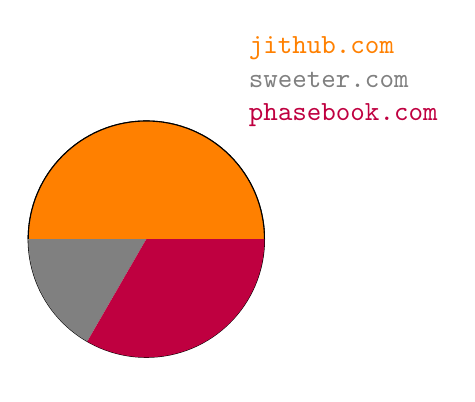
\begin{tikzpicture}
		\draw (0,0) circle [radius=1.5cm];
		\draw[fill=orange] (1.5, 0) arc [start angle = 0, end angle=180, radius =1.5cm];
		\fill[gray] (-1.5, 0) arc [start angle =180, end angle = 240, radius = 1.5] -- (0,0) --cycle;
		\fill[purple] (0,0) -- (-0.75, -1.3) arc [start angle = -120, end angle = 0,radius = 1.5cm] -- (1.5, 0) -- cycle;
		\node[align=left] at (2.5, 2) {\textcolor{orange}{\texttt{jithub.com}}\\\textcolor{gray}{\texttt{sweeter.com}}\\\textcolor{purple}{\texttt{phasebook.com}}};
	\end{tikzpicture}
	\caption{The ratio of teenagers' social networking activities in three platforms}
	\label{fig:piechart}
\end{figure}
\section*{Line graphs and talking about trends}
\begin{figure}
	\center
	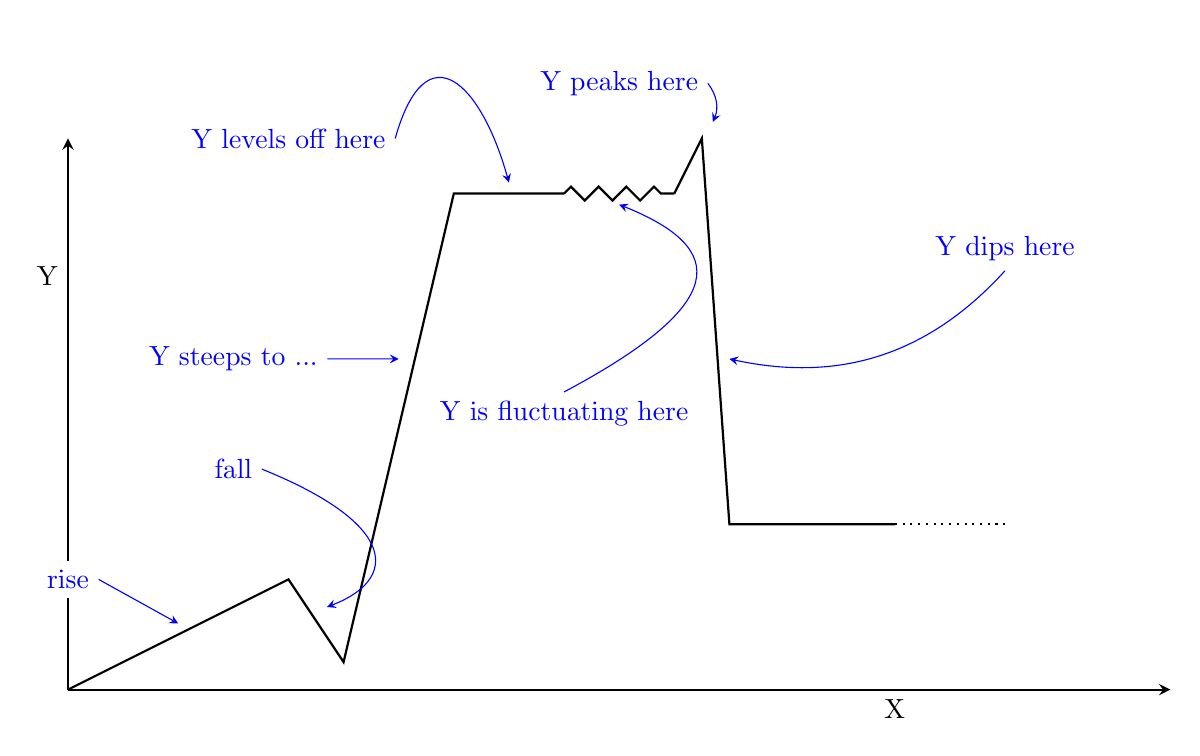
\begin{tikzpicture}[scale=0.7]
		\draw[-stealth, black, thick] (0,0) -- node[near end, below] {X} (20, 0);
		\draw[-stealth, black, thick] (0,0) -- node[near end, left] {Y}(0, 10);
		% \draw[very thin, gray] (0.1,0.1) grid (19.9,9.9);
		% \foreach \x in {1,...,20}
		% 	\node[below] at (\x, 0) {\x};
		% \foreach \y in {1,...,10}
			% \node[left] at (0, \y) {\y};
		\draw[thick] (0,0) -- (4,2) -- (5,0.5) -- (7,9) -- (9,9);
		\draw[thick, decorate, decoration=zigzag] (9,9) -- (11, 9);
		\draw[thick] (11, 9) -- (11.5, 10) -- (12, 3)--(15, 3);
		\draw[thick, dotted] (15,3) -- (17, 3);

		\node[fill=white, align=left] at (0, 2) (rise) {\textcolor{blue}{rise}};
		\draw[-stealth, blue ] (rise.east) -- (2, 1.2);

		\node[fill=white] at (3, 4) (fall) {\textcolor{blue}{fall}};
		\draw[-stealth, blue] (fall.east) .. controls (6, 3) and (6, 2) .. (4.7, 1.5);

		\node[fill=white] at (3, 6) (steep) {\textcolor{blue}{Y steeps to ...}};
		\draw[-stealth, blue] (steep.east) -- (6, 6);
		
		\node[fill=white] at (4, 10) (leveloff) {\textcolor{blue}{Y levels off here}};
		\draw[-stealth, blue] (leveloff.east) .. controls (6.5, 12) and (7.5, 11) .. (8, 9.2);

		\node[fill=white] at (9, 5) (fluctuate) {\textcolor{blue}{Y is fluctuating here}};
		\draw[-stealth, blue] (fluctuate.north) .. controls (12, 7) and (12, 8) .. (10, 8.8);

		\node[fill=white] at (10, 11) (peak) {\textcolor{blue}{Y peaks here}};
		\draw[-stealth, blue] (peak.east) to [bend left] (11.7, 10.3);

		\node[fill=white] at (17, 8) (dip) {\textcolor{blue}{Y dips here}};
		\draw[-stealth, blue] (dip.south) to [bend left] (12, 6);
	\end{tikzpicture}
	\caption{A sample line graph}
	\label{fig:linegraph}
\end{figure}
How something's changed over time can be effectively shown with a line graph (figure~\ref{fig:linegraph}). Here is some useful languge:
\begin{itemize}
	\item There was a[sharp, gradual, moderate, slight, steep] [rise, fall, ...] in ...
	\item Y [sharply, gradually, dramatically, ...] [rose, fell, dropped, ...]
	\item between ... and ...

		{\large \wela The academic interest in AI research decreased between 1974 and 1980.}
	\item over the following [X years, X days, ...]

		{\large \wela There was a significant rise in AI studies over the following seven years.}
\end{itemize}
\begin{framed}
\noindent \textcolor{red}{EXERCISE:} Before reading the caption and the text explanations for FIGURE 1.15 in the 4th edition of your textbook for \textbf{computer architecture} \cite{patterson}, take a look at the figure only. 
	\begin{framed}
\noindent 
\begin{tikzpicture} \draw[red, very thick] (0,0)--(0.25, 0.5)--(0.5,0)--cycle; \draw[red] (0.25, 0.35)--(0.25, 0.15); \draw[red] (0.25, 0.10) -- (0.25, 0.05); \end{tikzpicture} Only the figure, not the texts! 
	\end{framed}
	\noindent It plots the clock rate (in MHz) and power (in Watts) for a handful of Intel microprocessors. For each model, you see the two mentioned characteristics and the year the model was introduced. Paraphrase my explanation for the figure and write a couple of paragraphs about it. Do not include your opinions for why the data is this way, just be a passive narrator of the information given by the graph. Then compare what you have written with the explanations in the text. Send me your description and the text's analysis for the reason behind the statistics (in your own language of course, not copied!). 

\noindent \textcolor{red}{EXERCISE:} Repeat the previous exercise for FIGURE 1.1 of \cite{patterson}. It shows how many TVs, personal comptuers, and cellphones were manufactured each year in the U.S. over a priod of eleven years; from 1997 to 2007. TV data were availabe only from 2004.
\end{framed}
\bibliographystyle{apalike}
\bibliography{ref}
\end{document}
